\section{}
% Flow separates at a sharp corner along a wall and forms a recirculating 
% separation bubble as sketched below (streamlines are shown). The value of the 
% stream function at the wall is zero, and that of the uppermost streamline shown is 
% some positive value ψupper.
% Discuss the value of the stream function inside the separation bubble. In 
% particular, is it positive or negative? Why? Where in the flow is ψ a minimum?


Flow separates at a sharp corner along a wall and forms a recirculating separation bubble as sketched below (streamlines are shown). The value of the stream function at the wall is zero, and that of the uppermost streamline shown is some positive value $\psi_{\text{upper}}$. Discuss the value of the stream function inside the separation bubble. In particular, is it positive or negative? Why? Where in the flow is $\psi$ a minimum?

\begin{figure}[h]
    \centering
    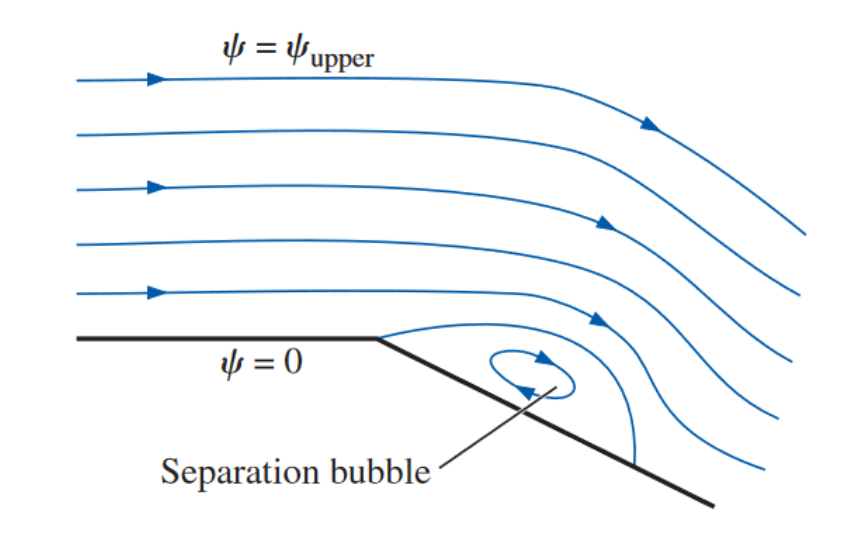
\includegraphics[width=0.5\textwidth]{Questions/Figures/q6 problem diagram.png}
    \caption{Flow separation}
\end{figure}

\subsection*{Solution}
Inside the seperation bubble, the stream is going in the clockwise direction. This corresponds to the tangential velocity being negative, $u_{\theta} < 0$. so the stream function is negative inside the separation bubble. 

The minimum value of the stream function occurs at the center of the separation bubble, where the velocity is zero. Thus, the stream function is a minimum at the center of the separation bubble.